\documentclass[10pt, a4paper, nofootinbib]{scrartcl}

\newcommand{\pagetitle}{LMAT1271 : Project report} 

\usepackage{amsmath}
\usepackage{amssymb}
\usepackage{amsthm}
\usepackage[T1]{fontenc}
\usepackage[french]{babel} % traduction
\usepackage[usenames,svgnames,dvipsnames]{xcolor}
%\usepackage{bookmark} 
%\usepackage{booktabs} % beautiful tables
%\usepackage[thicklines]{cancel} % cancel terms in equation
%\usepackage{color} % colors in box (theorems,...)
%\usepackage{enumerate}
\usepackage{float}
\usepackage{framed} % box around text
\usepackage{fancyhdr} % header
%\usepackage{fancyvrb}
\usepackage{mathtools}
\usepackage{mathrsfs}
\usepackage[parfill]{parskip} % avoid bad alignment in paragraphs
\usepackage{pgfplots} % plot in tikz
%\usepackage[arrowdel]{physics} % physics helpers (BUGGY)
\usepackage{derivative}
\usepackage{braket}
%\usepackage{setspace}
\usepackage{siunitx}
\usepackage{silence} % silence useless warnings
%\usepackage{systeme} % system of equations
\usepackage{tikz}
\usepackage{tkz-euclide}
\usepackage{tikz-3dplot}
\usepackage{units} % Non-stacked fractions and better unit spacing
\usepackage{xspace} % prints a trailing space in a smart way.
\usepackage{minted} % print code 

\usemintedstyle{monokay}

\usetikzlibrary{calc,patterns,angles,quotes}
\usetikzlibrary{hobby} % random curves with tikz

\tikzset{circ/.style = {fill, circle, inner sep = 0, minimum size = 3}}
\tikzset{scirc/.style = {fill, circle, inner sep = 0, minimum size = 1.5}}
\tikzset{mstate/.style={circle, draw, blue, text=black, minimum width=0.7cm}}

% \titlespacing*{\section}{0pt}{5.5ex plus 1ex minus .2ex}{4.3ex plus .2ex}
% \titlespacing*{\subsection}{0pt}{5.5ex plus 1ex minus .2ex}{4.3ex plus .2ex}

\usepackage{enumitem}
\setlist{nosep,after=\vspace{\baselineskip}}
% bullet instead of dash for items
\AtBeginDocument{\def\labelitemi{$\bullet$}}

\pgfplotsset{compat=1.12}
\sisetup{locale = FR}

\usepackage[marginparwidth=2cm]{geometry}
\geometry{
	paper=a4paper,
	inner=2.0cm,
	outer=3.0cm,
	bindingoffset=.5cm, 
	top=3.5cm, 
	bottom=3.5cm
}

\usepackage{graphicx}
\setkeys{Gin}{width=\linewidth,totalheight=\textheight,keepaspectratio}
%\graphicspath{{figures/}}

% Default images settings
\setkeys{Gin}{width=\linewidth, totalheight=\textheight, keepaspectratio}

\definecolor{blue}{rgb}{0,0,1}
\definecolor{red}{rgb}{1,0,0}

%------------------
% Théorèmes,...
%------------------
\usepackage{thmtools}
\usepackage[framemethod=TikZ]{mdframed}

\mdfdefinestyle{mdgreenbox}{%
	skipabove=8pt,
	linewidth=2pt,
	rightline=false,
	leftline=true,
	topline=false,
	bottomline=false,
	linecolor=ForestGreen,
	backgroundcolor=ForestGreen!5,
}
\declaretheoremstyle[
	headfont=\bfseries\sffamily\color{ForestGreen!70!black},
	bodyfont=\normalfont,
	postheadspace=\newline,
	spaceabove=2pt,
	spacebelow=1pt,
	mdframed={style=mdgreenbox},
	headpunct={ --- }
]{thmgreenbox}

\mdfdefinestyle{mdblackbox}{%
	skipabove=8pt,
	linewidth=3pt,
	rightline=false,
	leftline=true,
	topline=false,
	bottomline=false,
	linecolor=black,
	backgroundcolor=RedViolet!5!gray!5,
}
\declaretheoremstyle[
	headfont=\bfseries,
	bodyfont=\normalfont\small,
	spaceabove=0pt,
	spacebelow=0pt,
	mdframed={style=mdblackbox},
	postheadspace=\newline
]{thmblackbox}

\mdfdefinestyle{mdbluebox}{%
	roundcorner=10pt,
	linewidth=1pt,
	skipabove=12pt,
	innerbottommargin=9pt,
	skipbelow=1pt,
	nobreak=true,
	linecolor=blue,
	backgroundcolor=TealBlue!5,
}
\declaretheoremstyle[
	headfont=\sffamily\bfseries\color{MidnightBlue},
	mdframed={style=mdbluebox},
	headpunct={\\[3pt]}
]{thmbluebox}

\mdfdefinestyle{mdredbox}{%
	linewidth=0.5pt,
	skipabove=12pt,
	frametitleaboveskip=5pt,
	frametitlebelowskip=0pt,
	skipbelow=2pt,
	frametitlefont=\bfseries,
	innertopmargin=4pt,
	innerbottommargin=8pt,
	nobreak=true,
	linecolor=RawSienna,
	backgroundcolor=Salmon!5,
}
\declaretheoremstyle[
	headfont=\bfseries\color{RawSienna},
	mdframed={style=mdredbox},
	headpunct={\\[3pt]}
]{thmredbox}

\theoremstyle{definition}
\declaretheorem[name=Théorème,numberwithin=section,style=thmredbox]{theorem}
\declaretheorem[name=Définition,sibling=theorem,style=thmgreenbox]{definition}
\declaretheorem[name=Proposition,sibling=theorem,style=thmbluebox]{proposition}
\declaretheorem[name=Corollaire,sibling=theorem,style=thmbluebox]{corollary}
\declaretheorem[name=Lemme,sibling=theorem,style=thmbluebox]{lemma}
\declaretheorem[name=Exemple,sibling=theorem,style=thmblackbox]{example}
\declaretheorem[name=Question,sibling=theorem,style=thmblackbox]{ques}
\declaretheorem[name=Exercice,sibling=theorem,style=thmblackbox]{exercise}
\declaretheorem[name=Remarque,sibling=theorem,style=thmgreenbox]{remark}
\declaretheorem[name=Etape,style=thmgreenbox]{step}

%---------------------------------------------------
% BUGGY PACKAGES THAT NEED TO BE LOADED AT THE END
%---------------------------------------------------

% colored hyperlink
% load hyperref at the end to avoid conflicts
\usepackage[colorlinks]{hyperref} % colored ref
% % cleverref must be loaded after hyperref
% \usepackage{cleveref} % create ref

\hypersetup{
  colorlinks=true,
  linkcolor=blue,
  filecolor=blue,
  citecolor=black,
  urlcolor=cyan
}

% conditions for equations
% https://tex.stackexchange.com/questions/95838/how-to-write-a-perfect-equation-parameters-description
\newenvironment{conditions}
  {\par\vspace{\abovedisplayskip}\noindent\begin{tabular}{>{$}l<{$} @{${}={}$} l}}
	{\end{tabular}\par\vspace{\belowdisplayskip}}
	
\newenvironment{conditions*}
  {\par\vspace{\abovedisplayskip}\noindent
   \tabularx{\columnwidth}{>{$}l<{$} @{${}={}$} >{\raggedright\arraybackslash}X}}
  {\endtabularx\par\vspace{\belowdisplayskip}}

%----------------
% FIX
%----------------

\setlength{\headheight}{14.5pt}

% increase vertical space for aligned equations
\setlength{\jot}{7pt}

% Filter warnings issued by package biblatex starting with "Patching footnotes failed"
\WarningFilter{biblatex}{Patching footnotes failed}

%----------------------
%	COMMANDS
%----------------------

% commands shortcuts
\newcommand{\mb}{\mathbb}
\newcommand{\R}{\mb{R}}
\newcommand{\Z}{\mb{Z}}
\newcommand{\N}{\mb{N}}
\newcommand{\C}{\mb{C}}
\newcommand{\A}{\mb{A}} % hypersphere area
\newcommand{\V}{\mb{V}} % hypersphere volume
\newcommand{\dS}{\cdot d\vec{S}}
\newcommand{\lag}{\mathcal{L}}
\newcommand{\ham}{\mathcal{H}}
\newcommand{\Mod}[1]{\ \mathrm{mod}\ #1}
\newcommand{\res}{\text{res}}
\newcommand{\ind}{\text{ind}}
\newcommand{\carg}{\text{arg}}

\newcommand{\vb}[1]{\mathbf{\vec{#1}}} % bold vectors
\newcommand{\vd}[1]{\dot{\vec{#1}}} 
\newcommand{\vdd}[1]{\ddot{\vec{#1}}}

% norm
\newcommand{\bignorm}[1]{\left\lVert#1\right\rVert}

% smaller overline (line above variable)
\newcommand{\overbar}[1]{\mkern 1.5mu\overline{\mkern-1.5mu#1\mkern-1.5mu}\mkern 1.5mu}

% prints an asterisk that takes up no horizontal space.
% useful in tabular environments.
\newcommand{\hangstar}{\makebox[0pt][l]{*}}

% Prints argument within hanging parentheses (i.e., parentheses that take
% up no horizontal space). Useful in tabular environments.
\newcommand{\hangp}[1]{\makebox[0pt][r]{(}#1\makebox[0pt][l]{)}}

% cancel terms with color
% \newcommand{\ccancel}[2]{\renewcommand{\CancelColor}{\color{#2}}\bcancel{#1}}

% small parallel 
\makeatletter
\newcommand{\newparallel}{\mathrel{\mathpalette\new@parallel\relax}}
\newcommand{\new@parallel}[2]{%
  \begingroup
  \sbox\z@{$#1T$}% get the height of an uppercase letter
  \resizebox{!}{\ht\z@}{\raisebox{\depth}{$\m@th#1/\mkern-5mu/$}}%
  \endgroup
}
\makeatother

\renewcommand*\contentsname{Table des matières}
\usepackage{scrlayer-scrpage}
\pagestyle{scrheadings}

\setheadsepline{0.4pt} % Ligne au-dessus de la page
\setfootsepline{0.4pt} % Ligne au-dessous de la page

% header
\setkomafont{pagehead}{\bfseries}  % police en-tête 
\lohead{\pagetitle}  
\ohead{Mathieu Rousseau}

% footer
\ifoot{2020-2021}
\ofoot{\pagemark}

\pagenumbering{arabic}

\begin{document}

\section{Point estimation}

\subsection*{Context}
Our engineering team just landed a consulting contract with a company interested in the electricity consumption of its machines. In a first part, we would like to determine how electricity consumption is evenly distributed across the different machines of the same type. To this end, we use the Gini coefficient. In a nutshell, it is an index ranging from $0$ to $1$ measuring the inequality featured in a distribution. A value of $0$ denotes that all our machines use the same amount of electricity while a value of $1$ means that all the electricity is used by a single machine.
We assume that all of the $n$ machines operate independently and their daily electricity consumption (in MWh) can be modelled as a random variable $X$ with the following probability density function (PDF),

\begin{equation}
  f_{\theta_1, \theta_2}(x) = 
  \begin{cases}
    \frac{\theta_1 \theta_2^{\theta_1}}{x^{\theta_1 + 1}}, &\quad x \geq \theta_2 \\
    0,                                                     &\quad \text{otherwise}
  \end{cases}
\end{equation}

with $\theta_1 > 2$ and $\theta_2 > 0$. This is the PDF of the \textbf{Pareto distribution}.

\textbf{(a)} Derive the quantile function of $X$

\begin{center}\rule{6cm}{0.4pt}\end{center}

We're looking to solve $P(X \leq x_t) = t$ for $x_t$.

First let's compute the cumulative distribution function (CDFa) $P(X \leq x_t)$, 
\begin{align*}
  P(X \leq x_t)
    &= \int_{-\infty}^{x_t} f_{\theta_1, \theta_2}(x) dx \\
    &= \int_{\theta_2}^{x_t} \theta_1 \theta_2^{\theta_1} x^{-(\theta_1 + 1)} dx \\
    &= - \frac{\theta_1 \theta_2^{\theta_1}}{\theta_1} \left[ x^{-\theta_1} \right]_{x=\theta_2}^{x=x_t} \\
    &= - \theta_2^{\theta_1} \left( x_t^{-\theta_1} - \theta_2^{-\theta_1} \right) \\
    &= 1 - \left( \frac{\theta_2}{x_t} \right)^{\theta_1}
\end{align*}

Let's solve $P(X \leq x_t) = t$ for $x_t$,
\begin{align*}
  1 - \left( \frac{\theta_2}{x_t} \right)^{\theta_1} = t 
    &\iff (1 - t)^{1/\theta_1}
      = \frac{\theta_2}{x_t}\\
    &\iff x_t 
      = \frac{\theta_2}{(1 - t)^{1/\theta_1}}
\end{align*}

Therefore we have, 
\begin{equation}
  Q_{\theta_1, \theta_2}(t) = \frac{\theta_2}{(1 - t)^{1/\theta_1}}
\end{equation}

\textbf{(b)} Derive the Gini coefficient of $X$.

\begin{center}\rule{6cm}{0.4pt}\end{center}

The Gini coefficient is defined as, 
\begin{equation}
  G_{\theta_1, \theta_2} = 2 \int_{0}^{1} \left( p - \frac{\int_{0}^{p} Q(t) dt}{E(X)} \right) dp
\end{equation}

Let's first compute the expectation value of $X$,
\begin{align*}
  E(X)
    &= \int_{-\infty}^{+\infty} x \cdot f_{\theta_1, \theta_2}(x) dx \\
    &= \int_{\theta_2}^{+\infty} x \frac{\theta_1 \theta_2^{\theta_1}}{x^{\theta_1 + 1}} dx \\
    &= \theta_1 \theta_2^{\theta_1} \int_{\theta_2}^{+\infty} x^{- \theta_1} dx \\
    &= - \frac{\theta_1 \theta_2^{\theta_1}}{(\theta_1 - 1)} \left[ x^{-(\theta_1 - 1)} \right]_{\theta_2}^{+\infty} \\
    &= \begin{cases}
      - \frac{\theta_1 \theta_2^{\theta_1}}{(\theta_1 - 1)} \left( - \frac{1}{\theta_2^{-(\theta_1 - 1)}} \right), &\quad \theta_1 > 1 \\
      +\infty, &\quad \theta_1 \leq 1
    \end{cases} \\
    &= \begin{cases}
      \frac{\theta_1 \theta_2}{(\theta_1 - 1)}, &\quad \theta_1 > 1 \\
      +\infty, &\quad \theta_1 \leq 1
    \end{cases}
\end{align*}

So the Gini coefficient is defined for $\theta_1 > 1$, 
\begin{align*}
  G_{\theta_1, \theta_2}
    &= 2 \left( \int_{0}^{1} p dp - \int_{0}^{1} \frac{\int_{0}^{p} Q_{\theta_1, \theta_2}(t) dt}{E(X)} dp \right) 
\end{align*}

We compute each integral separately,
\begin{align*}
  \int_0^1 pdp 
    &= \frac{1}{2}
\end{align*}

Then,
\begin{align*}
  \int_0^p Q_{\theta_1, \theta_2}(t) dt 
    &= \theta_2 \int_0^p \frac{1}{(1 - t)^{1/\theta_1}}
\end{align*}

We use the change of variable $u = 1 - t \implies du = -dt$ 

The boundaries becomes, 
\begin{align*}
  \begin{cases}
    t = 0 &\implies u_1 \equiv 1 \\
    t = p &\implies u_2 \equiv 1 - p
  \end{cases}
\end{align*}

Then, 
\begin{align*}
  \int_0^p Q_{\theta_1, \theta_2}(t) dt 
    &= -\theta_2 \int_{u_1}^{u_2} \frac{1}{(u)^{1/\theta_1}} du \\
    &= -\theta_2 \left[ \frac{(u)^{-(1/\theta_1 - 1)}}{-((1/\theta_1) - 1)} \right]_{u_1}^{u_2} \\
    &= \frac{\theta_2}{(1/\theta_1) - 1} \left( \frac{1}{(1-p)^{1/\theta_1 - 1}} - \frac{1}{1^{1/\theta_1 - 1}} \right) \\
    &= \frac{\theta_2}{(1/\theta_1) - 1} \left( \frac{1}{(1-p)^{1/\theta_1 - 1}} - 1 \right)
\end{align*}

Therefore for $\theta_1 > 1$, 
\begin{align*}
  \frac{\int_{0}^{p} Q_{\theta_1, \theta_2}(t) dt}{E(X)}
    &= \frac{\frac{\theta_2}{(1/\theta_1) - 1} \left( \frac{1}{(1-p)^{1/\theta_1 - 1}} - 1 \right)}{\frac{\theta_1 \theta_2}{(\theta_1 - 1)}} \\
    &= \frac{\theta_2}{(1/\theta_1) - 1} \left( \frac{1}{(1-p)^{1/\theta_1 - 1}} - 1 \right) \frac{(\theta_1 - 1)}{\theta_1 \theta_2} \\
    &= \frac{\theta_1(1 - (1/\theta_1))}{((1/\theta_1) - 1)\theta_1} \left( \frac{1}{(1-p)^{1/\theta_1 - 1}} - 1 \right) \\
    &= - \left( \frac{1}{(1-p)^{(1/\theta_1) - 1}} - 1 \right) \\
    &= 1 - \frac{1}{(1-p)^{(1/\theta_1) - 1}}
\end{align*}

Then,
\begin{align*}
  \int_{0}^{1} \frac{\int_{0}^{p} Q_{\theta_1, \theta_2}(t) dt}{E(X)} dp 
    &= \underbrace{\int_0^1 1 dp}_{A} - \underbrace{\int_0^1 \frac{1}{(1-p)^{(1/\theta_1) - 1}} dp}_{B}
\end{align*}

Computing integral A and B.
\begin{align*}
  A = \int_0^1 1 dp = 1
\end{align*}

\begin{align*}
  B 
    &= \int_0^1 \frac{1}{(1-p)^{(1/\theta_1) - 1}} dp
\end{align*}

We use the change of variable $u = 1 - p \implies du = -dp$. 

The boundaries become, 
\begin{align*}
  \begin{cases}
    p = 0 &\implies u_1 \equiv 1 \\
    p = 1 &\implies u_2 \equiv 0
  \end{cases}
\end{align*}

Then, 
\begin{align*}
  \int_0^1 \frac{1}{(1-p)^{(1/\theta_1) - 1}} dp
    &= - \int_{u_1}^{u_2} \frac{1}{(u)^{(1/\theta_1) - 1}} du \\
    &= - \int_{u_1}^{u_2} u^{-((1/\theta_1) - 1)} du \\
    &= \frac{1}{((1/\theta_1) - 1) - 1} \left[ (u)^{((1/\theta_1) - 1 - 1)} \right]_1^0 \\
    &= -\frac{1}{(1/\theta_1) - 2} \\
    &= \frac{1}{2 - (1/\theta1)}
\end{align*}

Eventually the Gini coefficient is (for $\theta_1 > 0$),
\begin{align*}
  G_{\theta_1, \theta_2} 
    &= 2 \left( \frac{1}{2} - \frac{1}{2 - (1/\theta1)} \right) \\
    &= 2 \left( \frac{1}{2} \left[ 1 - \frac{1}{1 - (1/2\theta_1)} \right] \right) \\
    &= 1 - \frac{1}{1 - (1/2\theta_1)} \\
    &= \frac{1/2\theta_1}{1 - (1/2\theta_1} \\
    &= \frac{1}{2\theta_1 \left( 1 - \frac{1}{2\theta_1} \right)} \\
    &= \frac{1}{2\theta_1 - 1}
\end{align*}

\textbf{(c)} Derive the maximum likelihood estimator (MLE) of $G_{\theta_1, \theta_2}$. Call this estimator $\hat{G}_{\text{MLE}}$

\begin{center}\rule{6cm}{0.4pt}\end{center}

Let's first compute the likelihood function $L(\theta_1, \theta_2)$,
\begin{align*}
  L(\theta_1, \theta_2) 
    &:= \Pi_{i=1}^{n} f_{\theta_1, \theta_2} (x) \\
    &= \Pi_{i=1}^{n} \frac{\theta_1 \theta_2^{\theta_1}}{x^{\theta_1 + 1}} \cdot I(X_i \geq \theta_2 > 0) \\
    &= \theta_1^n \theta_2^{n\theta_1} \frac{1}{\Pi_{i=1}^{n} X_i^{\theta_1 + 1}} \cdot I(X_{(1)} \geq \theta_2 > 0) 
\end{align*}

where $X_{(1)} \equiv \min{(X_1,...,X_n)}$.

We notice that $L(\theta_1, \theta_2)$ is not continuous along $\theta_2$ and then not differentiable in $\theta_2$. However, we observe that $L(\theta_1, \theta_2)$ increase with $\theta_2$. Therefore, we have to take $\theta_2$ the largest possible in order to maximize $L(\theta_1, \theta_2)$ respecting the condition $X_{(1)} \leq \theta_2 > 0$ otherwise we would have $L(\theta_1, \theta_2) = 0$, 

\begin{equation*}
  \hat{\theta}_2 = X_{(1)}
\end{equation*}

For $\hat{\theta}_1$ we can compute the log-likelihood function $l(\theta_1, \theta_2)$, 
\begin{align*}
  l(\theta_1, \theta_2) 
    &:= \ln(L(\theta_1, \theta_2)) \\
    &= \ln(\theta_1^n) +  \ln(\theta_2^{n\theta_1}) + \ln(1) - \ln(\pi_{i=1}^{n} X_i^{(\theta_1 + 1)}) \\
    &= n\ln(\theta_1) + n\theta_1 \ln(\theta_2) - (\sum_{i=1}^{n} \ln(X_i^{(\theta_1 + 1)})) \\
    &= n\ln(\theta_1) + n\theta_1 \ln(\theta_2) - \sum_{i=1}^{n} (\theta_1 + 1))\ln(X_i)
\end{align*}

We differentiate with respect to $\theta_1$ in order to find the maximum,
\begin{align*}
  \pdv{l(\theta_1, \theta_2)}{\theta_1} 
    &= \frac{n}{\theta_1} + n\ln(\theta_2) - \sum_{i=1}^{n} \ln(X_i)
\end{align*}

Then, 
\begin{align*}
  \pdv{l(\theta_1, \theta_2)}{\theta_1} = 0 
    \iff \hat{\theta}_1 &= \frac{n}{\sum_{i=1}^{n} (\ln(X_i)) - n\ln(\hat{\theta}_2)} \\
                        &= \frac{n}{\sum_{i=1}^{n} (\ln(X_i) - \ln(X_{(1)}))} \\
                        &= \frac{n}{\sum_{i=1}^{n} \ln \left(\frac{X_i}{X_{(1)}} \right)} \\
\end{align*}

Now we can compute $\hat{G}_{\text{MLE}}$,
\begin{align*}
  \hat{G}_{\text{MLE}}
    &:= G_{\hat{\theta}_1, \hat{\theta}_2} \\
    &= \frac{1}{2\hat{\theta}_1 - 1} \\
    &= \frac{1}{\left( \frac{2n}{\sum_{i=1}^{n} \ln \left(\frac{X_i}{X_{(1)}} \right)} \right) - 1} 
\end{align*}

\textbf{(d)} Propose a method of moment estimator of $G_{\theta_1, \theta_2}$. Call this estimator $\hat{G}_{\text{MME}}$

\begin{center}\rule{6cm}{0.4pt}\end{center}

We already have computed the expectation value of $X$,
\begin{equation*}
  E(X) = 
    \begin{cases}
      \frac{\theta_1 \theta_2}{(\theta_1 - 1)}, &\quad \theta_1 > 1 \\
      +\infty, &\quad \theta_1 \leq 1
    \end{cases}
\end{equation*}

We know that, 
\begin{equation*}
  \bar{X} = \frac{1}{n} \sum_{i=1}^n X_i \equiv E(X)
\end{equation*}

Let's solve for $\theta_1$,
\begin{align*}
  \bar{X} = \frac{\hat{\theta}_1 \hat{\theta}_2}{(\hat{\theta}_1 - 1)} 
    \iff \bar{X} \hat{\theta}_1 - \bar{X} &= \hat{\theta}_1 \hat{\theta}_2 \\
    \iff \hat{\theta}_1 (\bar{X} - \hat{\theta}_2) &= \bar{X} \\
    \iff \hat{\theta}_1 &= \frac{\bar{X}}{(\bar{X} - \hat{\theta}_2)}
\end{align*}

In order to estimate $\hat{\theta}_2$ we know that the CDF is given by,
\begin{equation*}
  F_{\theta_1 \theta_2}(x) = P(X \leq x) = 1 - \left( \frac{\theta_2}{x} \right)^{\theta_1}
\end{equation*}

Therefore, 
\begin{align*}
  P(X > x) 
    &= 1 - P(X \leq x) \\
    &= \left( \frac{\theta_2}{x} \right)^{\theta_1}
\end{align*}

The probability that all random variables $(X_1, \dots, X_n)$ are greater than $x$ is, 
\begin{align*}
  P((X_1, \dots, X_n) > x) 
    &= \Pi_{i=1}^{n} P(X > x) \\
    &= \left( \frac{\theta_2}{x} \right)^{n \theta_1}
\end{align*}

Then, the probability that the minimum random variable $X_{(1)} \equiv \min(X_1,\dots,X_n)$ is greater than $x$ is also, 
\begin{align*}
  P(X_{(1)} > x) 
    &= \left( \frac{\theta_2}{x} \right)^{n \theta_1}
\end{align*}

Therefore, 
\begin{align*}
  P(X_{(1)} \leq x) 
    &= 1 - \left( \frac{\theta_2}{x} \right)^{n \theta_1}
\end{align*}

The corresponding probability density function is,
\begin{align*}
  f_{\theta_1, \theta_2}(x) 
    &= F'_{\theta_1, \theta_2}(x) \\
    &= \odv{}{x}\left(1 - \left( \frac{\theta_2}{x} \right)^{n \theta_1} \right) \\
    &= - \theta_2^{n\theta_1} \odv{}{x} \left( x^{-n\theta_1} \right) \\
    &= n\theta_1 \theta_2^{n\theta_1} x^{-(n\theta_1 + 1)} \\
    &= \frac{n\theta_1 \theta_2^{n\theta_1}}{x^{(n\theta_1 + 1)}}, \quad x \geq \theta_2
\end{align*}

The corresponding expectation value is,
\begin{align*}
  E(X) 
    &= \int_{\theta_2}^{+\infty} x \cdot f_{\theta_1, \theta_2}(x) dx \\
    &= \int_{\theta_2}^{+\infty} x \cdot \frac{n\theta_1 \theta_2^{n\theta_1}}{x^{(n\theta_1 + 1)}} dx \\
    &= n\theta_1 \theta_2^{n\theta_1} \int_{\theta_2}^{+\infty} x^{(-n\theta_1)} dx \\
    &= \frac{n\theta_1 \theta_2^{n\theta_1}}{-(n\theta_1 - 1)} \left( - \frac{1}{\theta_2^{-(n\theta_1 - 1)}} \right) \\
    &= \frac{n\theta_1 \theta_2}{(n\theta_1 - 1)}
\end{align*}

Setting expectation value $E(X)$ to be equal the minimum random variable $X_{(1)}$,
\begin{align*}
  X_{(1)} = \frac{n\theta_1 \theta_2}{(n\theta_1 - 1)} 
    \iff \hat{\theta}_2 = X_{(1)} \frac{(n \hat{\theta}_1 - 1)}{n\hat{\theta}_1} 
\end{align*}

Therefore, 
\begin{align*}
  \hat{\theta}_1 
    &= \frac{\bar{X}}{(\bar{X} - \hat{\theta}_2)} \\
    &= \frac{\bar{X}}{\bar{X} - X_{(1)}\frac{(n\bar{\theta}_1 - 1)}{n\hat{\theta}_1}} \\
  \iff \bar{X} 
    &= \hat{\theta}_1 \left( \bar{X} - X_{(1)}\frac{(n\bar{\theta}_1 - 1)}{n\hat{\theta}_1} \right) \\
    &=\hat{\theta}_1 \bar{X} - \hat{\theta}_1 X_{(1)}\frac{(n\bar{\theta}_1}{n\hat{\theta}_1} + \hat{\theta}_1 X_{(1)}\frac{1)}{n\hat{\theta}_1} \\
    &= \hat{\theta}_1 \left( \bar{X} - X_{(1)} \right) + \frac{X_{(1)}}{n} \\
  \iff \hat{\theta}_1 
    &= \frac{\bar{X} - (X_{(1)}/n)}{(\bar{X} - X_{(1)})} \\
    &= \frac{n\bar{X} - X_{(1)}}{n(\bar{X} - X_{(1)})}
\end{align*}

Now we can compute $\hat{G}_{\text{MME}}$,
\begin{align*}
  \hat{G}_{\text{MME}}
    &:= G_{\hat{\theta}_1, \hat{\theta}_2} \\
    &= \frac{1}{2\hat{\theta}_1 - 1} \\
    &= \frac{1}{\left( \frac{2(n\bar{X} - X_{(1)})}{n(\bar{X} - X_{(1)})} \right) - 1}
\end{align*}

\textbf{(e)} Set $\theta_1^0 = 3$ and $\theta_2^0 = 1$. Generate an i.i.d sample of size $n = 20$ from the density $f_{\theta_1^0, \theta_2^0}$. In order to achieve this, you can make use of the inverse transform sampling. Using this sample, compute $\hat{G}_{\text{MLE}}$ and $\hat{G}_{\text{MME}}$.

\begin{center}\rule{6cm}{0.4pt}\end{center}

We have,
\begin{equation*}
  f_{\theta_1^0, \theta_2^0} = 
  \begin{cases}
    \frac{3 \cdot 1^{3}}{x^{3 + 1}} = \frac{3}{x^4}, &\quad x \geq 1 \\
    0,                                &\quad \text{otherwise}
  \end{cases}
\end{equation*}

We compute the CDF of $X$,
\begin{align*}
  F_{\theta_1, \theta_2}(x) = \int_{1}^{x} \frac{3}{t^4} dt 
    &= 3 \left[ \frac{t^{-3}}{-3} \right]_1^{x} \\
    &= - \left( \frac{1}{x^3} - \frac{1}{1^3} \right) \\
    &= 1 - \frac{1}{x^3}
\end{align*}

The inverse is, 
\begin{align*}
  F^{-1}_{\theta_1, \theta_2}(y) 
    &= \frac{1}{(1-y)^{1/3}}
\end{align*}

Using the following R code,
\begin{minted}{R}
  source("src/utils.r")

  # set a seed for reproductability
  set.seed(42)

  # Generate sample of size n = 20 by using inverse transform sampling
  rv_vector <- inverse_transform_sampling(n = 20, inv_cdf = inv_cdf)

  # plot an histogram of the random variable vector
  hist(rv_vector, breaks = 50, freq = FALSE, xlab = "X", main = "random sample")

  # compute Gini coefficients
  gini_mle(rv_vector = rv_vector, n = 20)
  gini_mme(rv_vector = rv_vector, n = 20)
\end{minted}

We get the following estimations,
\begin{equation}
  \begin{array}{rl}
    \hat{G}_{\text{MLE}} = 0.1728057 \quad ; \quad \hat{G}_{\text{MME}} = 0.1770613
  \end{array}
\end{equation}

\textbf{(f)} Repeat this data generating process $N = 1000$ times (with the same sample size $n = 20$ and the same ($\theta_1^0$, $\theta_2^0$)). Hence, you obtain a sample of size $N$ of each estimator of $G_{\theta_1, \theta_2}$. Make a \textbf{histogram} and a \textbf{boxplot} of these two samples. What can you conclude ?

\begin{center}\rule{6cm}{0.4pt}\end{center}

\begin{minted}{R}
  # Generate N = 1000 times the sample
  x <- sim(N = 1000, n = 20, f = inverse_transform_sampling, inv_cdf)

  gini_mle_sample <- x["gini-mle-sample", ]
  gini_mme_sample <- x["gini-mme-sample", ]

  # histogram of gini samples
  par(mfrow = c(1, 2))
  hist(gini_mle_sample, breaks = 50, main = "", xlab = "Gini MLE sample", col = "steelblue")
  abline(v = gini_theoretical(theta_1), col = "green", lty = 2)
  hist(gini_mme_sample, breaks = 50, main = "", xlab = "Gini MME sample", col = "red")
  abline(v = gini_theoretical(theta_1), col = "green", lty = 2)
  legend("topright", c("Gini MLE", "Gini MME", "True Gini"), fill = c("steelblue", "red", "green"))

  # boxplot of gini samples
  par(mfrow = c(1, 2))
  boxplot(gini_mle_sample, col = "grey")
  abline(h = gini_theoretical(theta_1), col = "brown", lty = 2)
  boxplot(gini_mme_sample, col = "grey")
  abline(h = gini_theoretical(theta_1), col = "brown", lty = 2)
\end{minted}

\begin{figure}[H]
  \centering
  \includesvg{figures/gini_sample_histogram.svg}
  \caption{histogramme de $N = 1000$ simulations des coefficients de Gini estimé par la méthodes du maximum de vraisemblance (\textit{à gauche}) et la méthode des moments (\textit{à droite}) basées sur un échantillons de taille $n = 20$}
  \label{fig:gini-histogram-N=1000}
\end{figure}

\begin{figure}[H]
  \centering
  \includesvg{figures/gini_sample_boxplot.svg}
  \caption{boxplot de $N = 1000$ simulations des coefficients de Gini estimé par la méthodes du maximum de vraisemblance (\textit{à gauche}) et la méthode des moments (\textit{à droite}) basées sur un échantillons de taille $n = 20$}
  \label{fig:gini-boxplot-N=1000}
\end{figure}


\textbf{(g)} Use the samples obtained in (f) to estimate the \textbf{bias}, the \textbf{variance} and the \textbf{mean squared error (MSE)} of both estimators What can you conclude ?

\begin{center}\rule{6cm}{0.4pt}\end{center}

\textbf{(h)} Repeat the calculations in (f) for $n = 20$, $40$, $60$, $80$, $100$, $150$, $200$, $300$, $400$, $500$. Compare the \textbf{biases}, the \textbf{variances} and the \textbf{mean squared errors} of both estimators graphically (make a separate plot for each quantity as a function of $n$). What can you conclude ? Which estimator is the best ? Justify your answer.

\begin{center}\rule{6cm}{0.4pt}\end{center}

\textbf{(i)} Create an histogram for $\sqrt{n}(\hat{G}_{\text{MLE}} - G_{\theta_1^0, \theta_2^0} )$, for $n = 20$, $n = 100$ and $n = 500$. What can you conclude ?

\begin{center}\rule{6cm}{0.4pt}\end{center}

\section{Regression}

The company wants to understand how electricity consumption is linked to productivity (i.e daily amount in 1000 euros that the company gains when the machine operates). We gather a dataset made of $40$ independent observations for which we observe the following variables,
\begin{equation}
  \begin{array}{rl}
    X \equiv \text{Electricity consumption in MWh} \quad ; \quad Y \equiv \text{productivity in thousands of euros per day}
  \end{array}
\end{equation}

\textbf{(a)} Is it reasonnable to fit a linear regression model between \textbf{productivity} ($Y$) and \textbf{electricity consumption} ($X$) ? 
If no, what transformation of $X$ and/or $Y$ would you propose to retrieve a linear model ? Justify.

\underline{Hint}: graphical representation may help visualize how the variables and the residuals behave.

For the rest of the exercise, we work we the transformed variables $X^{\ast}$ and $Y^{\ast}$. 
Write down the obtained model.

\underline{Note}: it may be that $Y = Y^{\ast}$ and/or $X = X^{\ast}$.

\begin{center}\rule{6cm}{0.4pt}\end{center}

If we look at the scatter plot of X and Y. We see clearly that the relationship between X and Y is not linear at all.

\begin{figure}[H!]
  \centering
  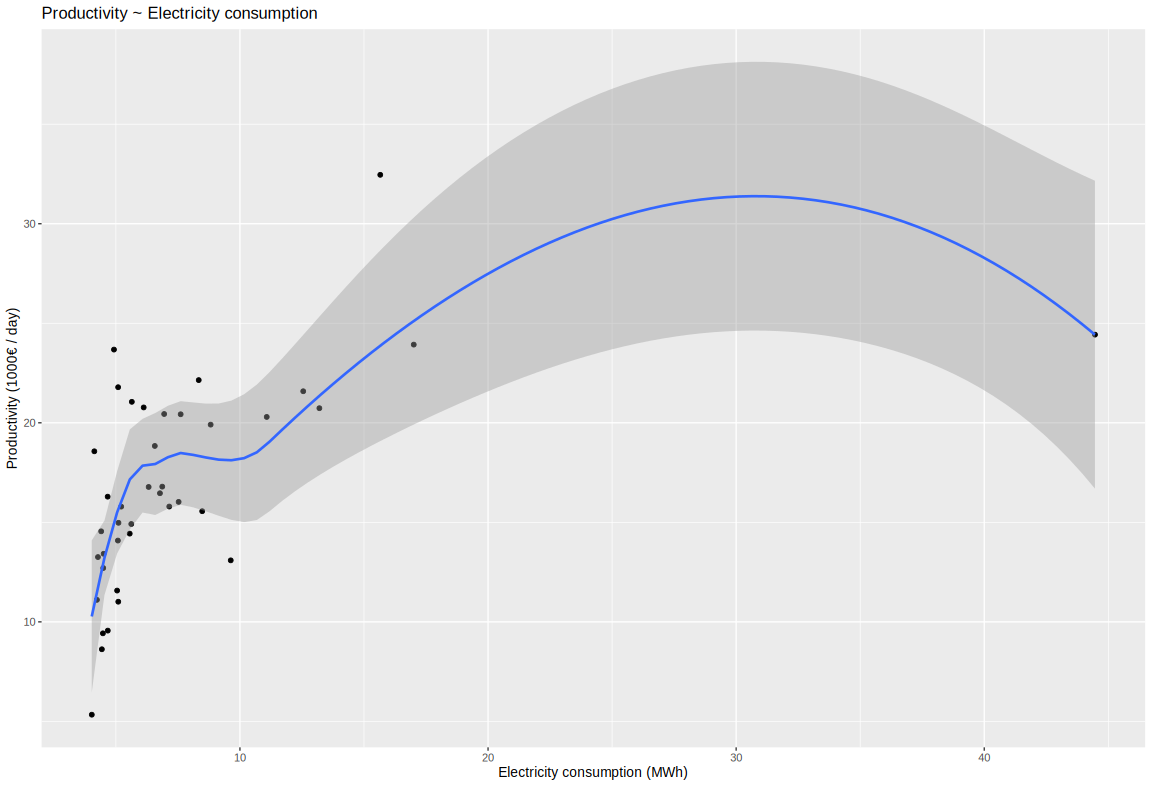
\includegraphics{../src/figures/scatter_plot.pdf}
  \caption{scatter plot of $X$ and $Y$}
  \label{fig:scatter_plot}
\end{figure}
 
\textbf{(b)} Mathematically derive the marginal impact of $X$ on $Y$ in your model. This is computed via the following formula, 
\begin{equation}
  \pdv{E(Y|X=x)}{x}
\end{equation}
Provide interpretation.

\begin{center}\rule{6cm}{0.4pt}\end{center}

\textbf{(c)} Is the linear effect significant ? Choose the adequate test for testing linear significance. Compute the p-value of this test. Based on the resulting p-value, what can we conclude ? Analyse the value of the linear effect.

\begin{center}\rule{6cm}{0.4pt}\end{center}

\newpage

\appendix
\appendixpage
\addappheadtotoc

\section{Code R: fichier utils.r}

\begin{minted}{R}
  theta_1 <- 3
  theta_2 <- 1

  # cumulative density function
  cdf <- function(x) {
    (-1 / x^3)
  }

  # inverse of cumulative density function
  inv_cdf <- function(y) {
    (1 / ((1 - y)^(1 / 3)))
  }

  # generate random variables vector from the inverse cdf
  inverse_transform_sampling <- function(n, inv_cdf) {
    # generate randoms numbers from the uniform distribution U(0,1)
    data_unif <- runif(n)
    rv_vector <- inv_cdf(y = data_unif)
  }

  # maximum likelihood method for gini coefficient estimator
  gini_mle <- function(rv_vector, n) {
    return(1 / ((2 * n) / (sum(log(rv_vector / min(rv_vector)))) - 1))
  }

  # method of moment for gini coefficient estimator
  gini_mme <- function(rv_vector, n) {
    return(1 / ((2 * (n) * mean(rv_vector) - min(rv_vector)) / (n * (mean(rv_vector) - min(rv_vector))) - 1))
  }

  gini_theoretical <- function(theta_1) {
    return(1 / ((2 * theta_1) - 1))
  }

  bias <- function(sample, theoretical) {
    mean(sample) - theoretical
  }

  mse <- function(sample, theoretical) {
    mean((sample - theoretical)^2)
  }

  # x: simulation of sample size n
  compute_statistical_quantities <- function(x, n) {
    mean <- mean(x)

    gini_mle_estimator <- gini_mle(rv_vector = x, n = n)
    gini_mme_estimator <- gini_mme(rv_vector = x, n = n)

    print(gini_mle_estimator)
    print("next simulation")

    c(
      mean,
      gini_mle_estimator,
      gini_mme_estimator
    )
  }

  # N: simulation size (i.e. number of samples)
  # n: sample size
  # f: function to generate random variables
  # ... any other parameters given to f
  sim <- function(N = 1000, n = 20, f, ...) {
    # compute a matrix of random variables based on the distribution f
    # each column correspond to one simulation
    x <- matrix(f(N * n, ...), nrow = n)

    # for each column (i.e. each simulation of sample size n)
    # we compute statistical quantities (mean, gini estimators,...)
    # the function "FUN" is called for each column
    stats <- apply(
      X = x,
      MARGIN = 2,
      FUN = compute_statistical_quantities,
      n = n
    )

    rownames(stats) <- c("mean-sample", "gini-mle-sample", "gini-mme-sample")

    return(stats)
  }
\end{minted}

\end{document}
